% Executive summary (read this first): Parked study-protocol draft for a blinded rationale-provenance audit. It is not the current paper proposal; see docs/PROPOSAL.md. No study results are claimed.
\documentclass[10pt]{article}
\usepackage[margin=0.85in]{geometry}
\usepackage[T1]{fontenc}
\usepackage{lmodern}
\usepackage{microtype}
\usepackage{booktabs}
\usepackage{hyperref}
\usepackage{enumitem}
\usepackage{tikz}
\usetikzlibrary{arrows.meta,positioning}
\hypersetup{colorlinks=true, linkcolor=blue, citecolor=blue, urlcolor=blue}
\title{Can You Tell How the Forecast Was Made?\\A Blinded Provenance Audit for Probabilistic Finance Forecasts}
\author{Draft for discussion\\[2pt]\small Agenthon 2026 workshop submission}
\date{\today}

\begin{document}
\maketitle

\begin{abstract}
Probabilistic forecasts can be numerically useful while their accompanying rationales are difficult to audit. A rationale may be generated as part of the forecasting process, or written after a forecast has already been fixed. These two artifacts can look equally coherent, yet support different claims about how the forecast was produced. We propose a blinded, matched-pair study in quantitative-finance forecasting: for each task, timestamped evidence packet, and forecast distribution, construct one rationale under a forecast-first procedure and one under an answer-first procedure. Independent reviewers see only one member of each pair and judge which provenance is more likely. The protocol targets 60 unique pairs balanced across four Agenthon Track 2 task families, with 12 human reviewers. It measures discrimination, false accusations against forecast-first rationales, reviewer agreement, and confidence calibration. The study tests whether construction-order cues are detectable in released artifacts; it does not establish whether a model's private reasoning caused its forecast. No results are reported here. We specify controls, analysis, and an artifact-history plan so the experiment can be preregistered and reproduced before any empirical claim is made.
\end{abstract}

\section{Introduction}
Forecasting systems increasingly return both a distribution over future outcomes and a natural-language explanation. In finance, the explanation can help an analyst inspect assumptions, connect a forecast to dated evidence, and identify disagreement. But a polished explanation is not automatically evidence that the forecast was derived from the stated reasoning.

This creates a simple audit question: given the same information and exactly the same forecast, can an independent reviewer tell whether the rationale was produced before or after that forecast was fixed? We call the first construction \emph{forecast-first} and the second \emph{answer-first}. The distinction concerns an observable generation procedure. It is deliberately narrower than the broad and often unobservable question of whether a model's internal chain of thought is faithful.

We propose a controlled test using Agenthon Track 2, which combines time-series forecasting with a frozen, timestamped text corpus. Matched cases hold the evidence and forecast distribution constant while varying the documented rationale-generation order. Reviewers are blinded to labels and pair membership and never see both rationales for one case. Our main outcome is their ability to discriminate the two construction procedures without falsely flagging forecast-first rationales.

\paragraph{Contributions sought.} This work would contribute (1) a paired protocol for auditing provenance cues in finance forecast rationales, (2) a blinded human evaluation that measures both detection and false accusation, and (3) a reproducible research artifact linking each claim to data references, prompts, code revisions, and analysis outputs. These are proposed contributions, not findings. ARA-style artifact practice is a reproducibility design choice, not a novelty claim of this paper \cite{liu2026ara}.

\section{Related work and positioning}
Work on reasoning faithfulness has developed benchmarks that compare explanations with controlled interventions and alternative evidence. FaithCoT-Bench studies instance-level chain-of-thought unfaithfulness across models and domains \cite{faithcot}. Recent forecasting benchmarks evaluate reasoning together with forecast quality, including finance settings \cite{tfrbench}. Other work reports cases where changing evidence can move a forecast without changing its accompanying rationale \cite{knowdontsay}. These studies motivate evaluating the relationship between forecasts, evidence, and explanations, but do not by themselves answer our narrower blinded provenance question.

Recent counterfactual tests also probe whether explanations track changes in model outputs \cite{counterfactualcot}. For time series, interpretable forecasting work studies explanation quality and model behavior \cite{ibforecast}; large-scale forecasting studies relate written rationales to human judgment quality \cite{fri}. MUSE-Bench expands multimodal, timestamped-context evaluation, including financial tasks \cite{muse}. Together this literature makes a broad claim such as “we are the first to test forecasting explanations” untenable.

Our candidate gap is more specific: a matched, reviewer-blinded comparison in which the visible evidence packet and forecast distribution are held exactly fixed, and the known difference is whether the rationale was generated before or after the forecast was fixed. A literature search cannot prove that no prior work uses this exact protocol. The claim should therefore remain “we study” unless a final systematic search establishes stronger priority.

\section{Research question and hypotheses}
\textbf{RQ:} Can human reviewers infer rationale construction order from the visible forecast-and-rationale artifact, when the evidence packet and forecast distribution are identical within each matched pair?

\textbf{H1 (discrimination):} Reviewers discriminate answer-first from forecast-first rationales above chance on held-out matched cases.

\textbf{H2 (specificity):} Any discrimination is not achieved by indiscriminately labeling rationales answer-first; the false-positive rate on forecast-first cases remains acceptably low.

\textbf{H3 (uncertainty):} Reviewer confidence is informative about correctness, assessed with a proper scoring rule and calibration summaries.

H1--H3 are hypotheses to preregister, not established outcomes. Before data collection, we must define “acceptably low” for H2 with the intended use and audience in mind. We do not assume a universal safety threshold.

\section{Study design}
\subsection{Unit and paired construction}
The unit is a forecasting case: a task specification, as-of timestamp, frozen evidence packet, forecast target and horizon, and forecast distribution. Each pair shares the same visible case and forecast object. It contains two rationales:
\begin{enumerate}[leftmargin=*]
\item \textbf{Forecast-first:} a generator receives the task and evidence, produces a forecast distribution, and records its rationale under a prespecified format.
\item \textbf{Answer-first:} after that forecast distribution has been frozen, a generator receives the same task and evidence plus the fixed distribution and writes a rationale consistent with it.
\end{enumerate}
For both conditions, retain the exact prompt, model and version, decoding settings, run identifier, evidence manifest, timestamps, and hashes in a restricted generation record. Match generator family and formatting wherever feasible; block on generator family and card family in sampling. Any unavoidable difference must be documented before unblinding.

The manipulation is the information and order specified in the generation procedure. It is not a direct measurement of hidden model cognition. In particular, a forecast-first rationale can still be post-hoc in a psychological sense, and an answer-first rationale can be indistinguishable if it contains no detectable cues.

\subsection{Sample and reviewers}
The provisional target is 60 unique pairs, 15 per Track 2 family (F1--F4). Sample distinct historical episodes rather than paraphrases of one episode. Use at least two forecast/rationale generator families if access permits, with family and generator balanced across task families. This target is a design proposal; cases and reviewers are not yet secured.

Recruit 12 human reviewers with relevant quantitative, forecasting, or machine-learning experience. Assign six reviewers to each pair: three see its forecast-first member and three its answer-first member. Each reviewer sees 30 cases, one per pair in their assigned subset. A reviewer never sees both members of a pair. Randomize case order and remove provenance labels, pair IDs, and generator identity. Record eligibility, expertise, exclusions, missing ratings, and compensation before recruitment.

\subsection{Reviewer task and outcomes}
For each case, show the forecast, rationale, and the same dated evidence available to the generator. Ask: “Was this rationale written after the forecast distribution had already been fixed?” Collect a binary judgment and confidence from 0 to 100. Lock responses before revealing labels or pair links.

The primary outcomes are reviewer-level balanced accuracy and AUROC (using confidence as the continuous score), with uncertainty intervals that respect clustering by case and reviewer. Report the false-positive rate on forecast-first cases separately from sensitivity on answer-first cases. Secondary outcomes include confidence calibration, inter-reviewer agreement, and variation by task family and generator family. LLM reviewers, if included, are a separate secondary analysis and are not pooled with humans.

\subsection{Assignment and blinding}
An assignment script validates that each pair has exactly one item from each condition and that the evidence and forecast objects match byte-for-byte after canonical serialization. It selects a balanced subset of reviewers per pair, hides labels and pair IDs, randomizes order, and writes a separate key. The key and generation records remain inaccessible to reviewers and analysis code until judgments are locked. Exclusions and any deviations are logged before unblinding.

\begin{figure}[t]
\centering
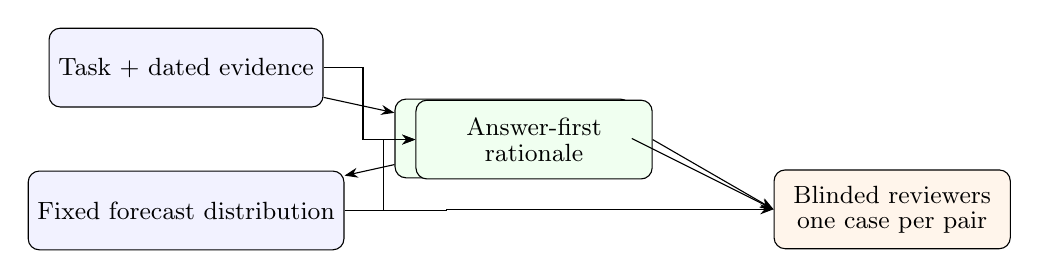
\begin{tikzpicture}[>=Stealth, node distance=8mm and 9mm,
  box/.style={draw, rounded corners, align=center, minimum width=30mm, minimum height=10mm, font=\small},
  shared/.style={box, fill=blue!5}, route/.style={box, fill=green!6},
  reviewer/.style={box, fill=orange!8}]
  \node[shared] (e) {Task + dated evidence};
  \node[shared, below=of e] (f) {Fixed forecast distribution};
  \node[route, right=of e, yshift=-9mm] (pre) {\shortstack{Forecast-first\\rationale}};
  \node[route, right=of f, yshift=9mm] (post) {\shortstack{Answer-first\\rationale}};
  \node[reviewer, right=18mm of pre, yshift=-9mm] (blind) {\shortstack{Blinded reviewers\\one case per pair}};
  \draw[->] (e) -- (pre);
  \draw[->] (pre) -- (f);
  \draw[->] (e.east) -- ++(5mm,0) |- (post.west);
  \draw[->] (f.east) -- ++(5mm,0) |- (post.west);
  \draw[->] (f.east) -- ++(13mm,0) |- (blind.west);
  \draw[->] (pre.east) -- (blind.west);
  \draw[->] (post.east) -- (blind.west);
  \end{tikzpicture}
\caption{Proposed paired protocol. Both conditions share the task, evidence, and exact forecast distribution. The reviewer sees a randomized single case and does not see its pair. The diagram describes procedure, not empirical evidence.}
\label{fig:design}
\end{figure}

\section{Analysis plan}
Freeze the analysis code and assignment seed before unblinding. Report the number of unique cases and ratings separately. Estimate balanced accuracy, AUROC, sensitivity, false-positive rate, and calibration with intervals that resample or model both case and reviewer dependence. Do not treat 360 ratings as 360 independent cases. Provide per-reviewer and per-family estimates alongside aggregate summaries.

For the false-positive rate, report the exact binomial interval over unique forecast-first traces as a transparent descriptive bound, while noting that traces are not truly independent if they share episodes, generators, or templates. With zero false positives among 60 independent traces, the one-sided exact 95\% upper bound is approximately 4.9\%; this is a planning calculation, not a result. Use pair- and reviewer-clustered uncertainty for discrimination metrics. Any automated detector must be trained on a separate development set and evaluated on held-out cases and, where possible, a held-out generator family.

\section{Validity, ethics, and limitations}
The most important limitation is construct validity: reviewers may detect stylistic artifacts of the prompt or generation pipeline rather than meaningful provenance. Matching, masking generator identity, and balancing families reduce but do not eliminate this risk. The protocol tests detectability of a documented construction order in released artifacts; it cannot prove a model's internal causal process, detect every form of post-hoc explanation, or establish that a rationale faithfully represents computation.

The proposed sample is modest, especially for subgroup analysis. The 60-pair target offers a useful first controlled study, not definitive coverage of models, markets, languages, or task types. Realized outcomes must not leak into generation prompts or reviewer packets. Reviewers should be told that the task evaluates artifacts rather than people, and results should not be used to accuse individual teams without independent evidence and due process.

\section{Reproducibility and artifact history}
The released package should contain the protocol, public-safe case manifests, assignment and analysis code, prompts, dependency lock, run instructions, and claim-to-evidence index. For every reported claim, record the source reference, code revision, configuration, command, output hash, and analysis. Preserve unsuccessful runs and changes in a dated history so readers can reconstruct how the analysis evolved. Keep restricted keys, private test material, and any protected data outside the public package. We will use the principles of agent-native research artifacts as an implementation guide, while evaluating this study on its own scientific contribution \cite{liu2026ara}.

\section{Conclusion}
We have specified a blinded, matched-pair experiment for one narrow question: whether people can infer that a finance forecast rationale was written after its forecast was fixed, when the visible evidence and forecast are held constant. The design makes false accusations and uncertainty first-class outcomes. Its value depends on executing the preregistered study, reporting null or ambiguous results, and preserving enough history for independent reconstruction. Until those steps are complete, this paper is a proposal rather than evidence that provenance can be detected.

\begin{thebibliography}{9}
\bibitem{faithcot} FaithCoT-Bench: Instance-Level Evaluation of Chain-of-Thought Faithfulness. ICLR 2026. \url{https://arxiv.org/abs/2510.04040}
\bibitem{tfrbench} TFRBench: A Reasoning Benchmark for Evaluating Forecasting Systems. ICML 2026. \url{https://arxiv.org/abs/2604.05364}
\bibitem{knowdontsay} What LLM Forecasters Know but Don't Say: Evidence Sensitivity and Rationale Stability. 2026. \url{https://arxiv.org/abs/2607.08046}
\bibitem{counterfactualcot} Counterfactual Tests for Chain-of-Thought Faithfulness in Vision Models. 2026. \url{https://arxiv.org/abs/2609.06704}
\bibitem{ibforecast} IB-Forecast: Interpretable Time-Series Forecasting. 2026. \url{https://arxiv.org/abs/2607.28124}
\bibitem{fri} Forecasting Research Institute. Measuring Judgment Quality in Forecasting Tournaments. 2026. \url{https://forecastingresearch.org/research/measuring-judgment-quality-forecasting-tournaments}
\bibitem{muse} MUSE-Bench: A Multimodal Benchmark for Forecasting with Heterogeneous Context. 2026. \url{https://arxiv.org/abs/2609.15087}
\bibitem{liu2026ara} J. Liu et al. The Last Human-Written Paper: Agent-Native Research Artifacts. 2026. \url{https://arxiv.org/abs/2604.24658}
\end{thebibliography}
\end{document}
